\documentclass[12pt]{article}
\usepackage[margin=1 in]{geometry}
\usepackage{graphicx}
\usepackage{float}
\usepackage{booktabs}
\usepackage{siunitx}
\usepackage{amsmath}
\usepackage{amssymb}


\title{Lab 9: Introduction to RC Circuits in the Time and Frequency-Domains}
\author{Sean Balbale}
\date{November 8th, 2024}
\setlength{\parindent}{0in}

\begin{document}

\begin{titlepage}
	\begin{center}
		\vspace*{1in}

		\Huge
		\textbf{Lab 9}

		\LARGE
		Introduction to RC Circuits in the Time and Frequency-Domains

		\vspace{3 in}

		\textbf{Student Name:} Sean Balbale
		\\ \textbf{Instructor:} Dr. Iman Salama
		\\ \textbf{Lab Partner Name:} Krish Gupta
		\\ \textbf{Date:} November 8, 2024

		\vfill


	\end{center}
\end{titlepage}

\newpage

\section{Introduction} 
This lab explored the behavior of RC (resistor-capacitor) circuits in 
time and frequency domains to understand their response to different 
input signals, essential in applications like signal processing and 
filtering. In Section \ref{subsec:part 1}, the transient response of 
an RC circuit was 
investigated using a square wave input to observe the exponential 
charging and discharging of the capacitor, governed by the time 
constant \(\tau = RC\). Adjustments in input frequency enabled full 
charge and discharge cycles, revealing insights into the circuit's 
time-domain behavior. Section \ref{subsec:part 2} analyzed the frequency 
response with a 
sine wave input across various frequencies, demonstrating 
frequency-dependent changes in output voltage magnitude and phase 
shift. These findings provided a foundational understanding of 
RC circuits’ responses across different conditions.


\section{Results}
% \begin{figure}[H]
% 	\centering
% 	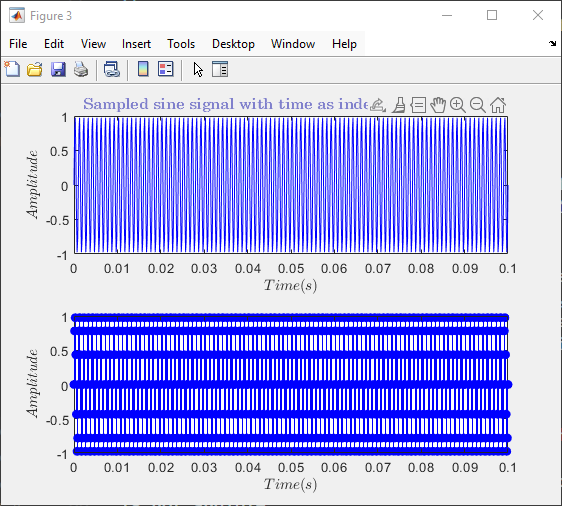
\includegraphics[width=0.3\textwidth]{fig 1f 7000.png}\hfill
% 	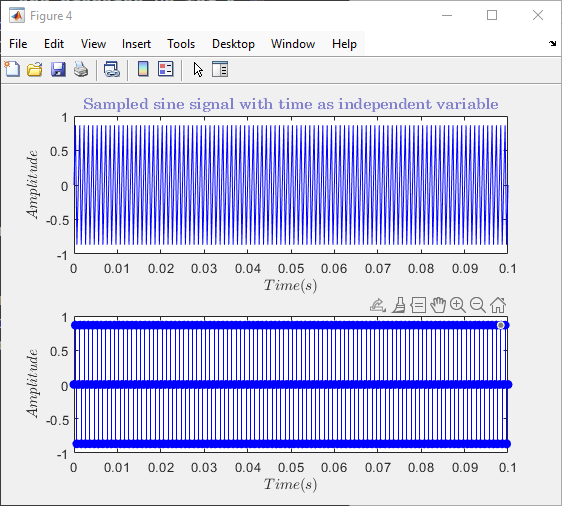
\includegraphics[width=0.3\textwidth]{fig 1f 3000.png}\hfill
% 	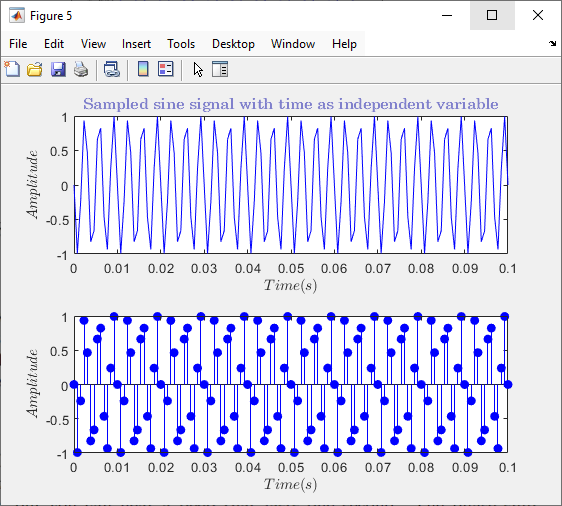
\includegraphics[width=0.3\textwidth]{fig 1f 1300.png}
% 	\caption{Sinusoidal with $f_s$ = 7 kHz, 3 kHz, and 1.3 kHz}
% 	\label{fig:fig3}
% % \end{figure}
\subsection{Transient Signals with an RC Circuit with Square Waves} \label{subsec:part 1}
The circuit consisted of a \SI{20}{\kilo\ohm} resistor in series with a \SI{0.1}{\micro\farad} capacitor, as
shown in Figure \ref{fig:simpleRCCircuit}. A function generator provided a 1 V amplitude square wave
with a 1 V DC offset, switching between 2 V and 0 V. The oscilloscope was used
to observe the voltage across the capacitor.

\begin{figure}[H]
	\centering
	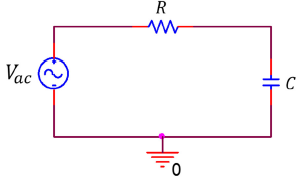
\includegraphics[width=0.5\textwidth]{SimpleRCCircuit.png}
	\caption{Simple RC Circuit}
	\label{fig:simpleRCCircuit}
\end{figure}

The cirucit was built was built with a \SI{19.790}{\kilo\ohm} resistor 
and a \SI{0.107}{\micro\farad} capacitor. The time constant was 
calculated to be:
\[
\tau = R \cdot C = 20000 \cdot 0.0000001 = 0.002
\]

A function generator was used to provide a square wave input with a frequency of $\frac{1}{10 \tau}$.
The oscilloscope was used to measure the voltage across the 
capacitor. This results in the following decay curve:

\begin{figure}[H]
	\centering
	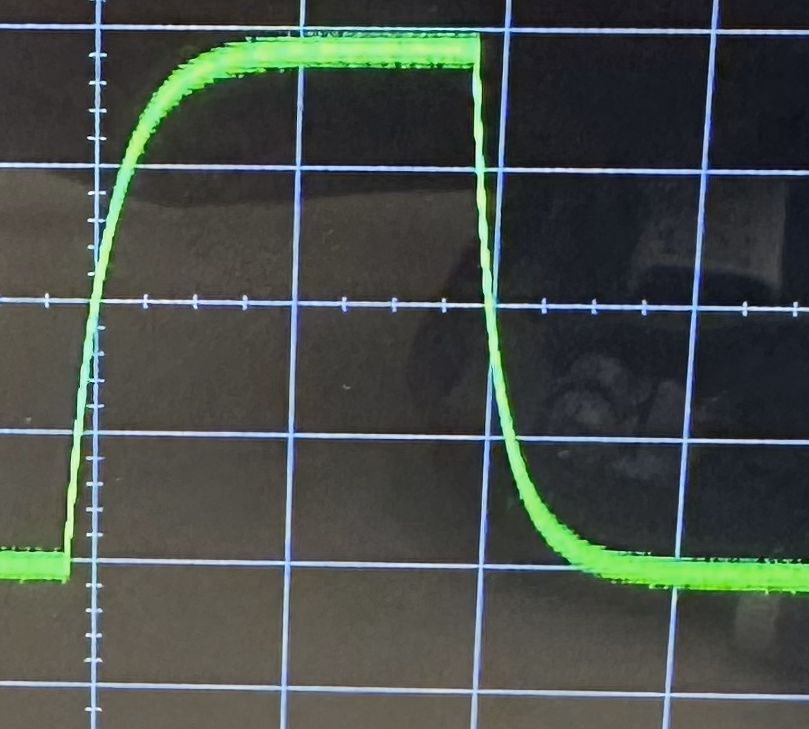
\includegraphics[width=0.5\textwidth]{decayfunction.png}
	\caption{Decay Curve}
	\label{fig:decayCurve}
\end{figure}

The decay curve was used to calculate the time constant of 
the circuit. The time constant was calculated from the following
equation:
\[
V(t) = V_0 \cdot e^{-\frac{t}{\tau}}
\]
$v_0$ was measured at 20 ms. From the decay curve (Figure \ref{fig:decayCurve}), 
$V_0 = 1.844$ V, and $V(t) = 0.975$ V. The time was found to be
$t_{top} - t_{chosen} = 0.0186 - 0.02$.
Thus the equation becomes:
\begin{align*}
	v_c (t) &= v_0 \cdot e^{-\frac{t_{top} - t_{chosen}}{\tau}} \\
	0.975 &= 1.844 \cdot e^{-\frac{0.0186 - 0.02}{\tau}} \\
	\therefore \tau &= 0.0021
\end{align*}
This is close to the theoretical time constant of 0.002 and within an acceptable 
range of error.

\subsection{A Simple RC Circuit with Sine Waves} \label{subsec:part 2}
The function generator is hooked up to the circuit and an 
oscilloscope. The function generator provides a 1 V amplitude
sine wave at a frequency ($f$) of 80 Hz. The circuit has the 
same 80 Hz frequency as the input, however the phase ($\phi$)
is different by 2 ms. we can calculate this in radians by the 
following equation:
\begin{align*}
	\Delta \phi &= (2 \pi)\cdot f \cdot \Delta t \\
				&= (2 \pi) \cdot 80 \cdot 0.002 \\
				&= \frac{8 \pi}{25}
\end{align*}
	
With the same RC circuit, a 1 V amplitude sine wave was applied at various
frequencies. The output voltage across the capacitor was measured at frequencies
of 80 Hz, 100 Hz, 1000 Hz, and 10000 Hz, and then at lower frequencies of 10 Hz,
1 Hz, and 0.1 Hz.
\newline

The phase shift was calculated for all these frequencies. For the lower frequencies 
of 10 Hz, 1 Hz, and 0.1 Hz, the phase shift was not calculated as the oscilloscope 
was unable to measure the value of $\Delta t$.
\begin{table}[H]
    \centering
    \begin{tabular}{|c|c|c|c|}
        \hline
        Frequency (Hz) & $\Delta t$ (ms) & Amplitude (V) & Phase ($\Delta \phi$) \\
        \hline
        80    & 2    	& 0.8 	& $\frac{8 \pi}{25}$ \\
        \hline
        100   & 16   	& 0.7 	& $\frac{8 \pi}{25}$\\
        \hline
        1000  & 0.26  	& 0.125 & $\frac{13 \pi}{25}$ \\
        \hline
        10000 & 0.0236  & 0.006 & $\frac{59 \pi}{1250}$ \\
        \hline
        10    & -   	& 1.07 	& - \\
        \hline
        1     & -   	& 1.21 	& - \\
        \hline
        0.1   & -   	& 1.30 	& - \\
        \hline
    \end{tabular}
    \caption{Frequency, $\Delta t$, Amplitude, and Phase}
    \label{tab:frequency_phase}
\end{table}

From the data in Table \ref{tab:frequency_phase}, we can see that as the frequency
approaches 0, the amplitude of the output voltage increases and the phase shift decreases.
Conversely, as the frequency approaches infinity, the amplitude of the output 
voltage decreases and the phase shift increases.

\section{Discussion and Conclusion}

In this lab, we explored the fundamental behaviors of RC circuits in both the time and frequency domains, providing insight into their applications in signal processing and filtering. Using a square wave input, the transient response of the RC circuit demonstrated the charging and discharging behavior of the capacitor, defined by the time constant \( \tau = RC \). Our experimental results for \( \tau \) were consistent with the theoretical calculations, affirming the exponential nature of capacitor charging and discharging in response to step inputs.
\newline

The frequency-domain analysis further highlighted the RC circuit’s role as a low-pass filter. At lower frequencies, the output amplitude remained high and closely matched the input, with minimal phase shift, indicating the circuit’s ability to pass low-frequency signals with little attenuation. As the input frequency increased, however, the output amplitude decreased, and the phase lag between the input and output signals increased. This behavior results from the increasing capacitive reactance, which filters out higher frequency components, thus demonstrating the filtering capabilities of the RC circuit.
\newline

In summary, this lab reinforced theoretical expectations regarding RC circuits in both the time and frequency domains. By observing how the output varies with different input waveforms and frequencies, we gained a practical understanding of RC circuit dynamics. These foundational principles are critical in fields such as biomedical signal processing, where RC circuits are used to filter out noise and enhance signal quality. This experiment serves as a basis for more complex analyses in future studies, including phasor-domain analysis and advanced filter design.


\section{References}
 [1] Dr. Iman Salama. “Lab 9 – Introduction to RC Circuits in the Time and Frequency-Domains” Northeastern University. 8 November 2024.

\end{document}
